\documentclass[10pt,a4paper]{article}
\usepackage[margin=1.1cm,top=1.2cm,bottom=1.2cm]{geometry}
\usepackage{amsmath,amssymb,amsfonts}
\usepackage{tcolorbox}
\tcbuselibrary{skins,breakable}
\usepackage{booktabs}
\usepackage{tabularx}
\usepackage{colortbl}
\usepackage{xcolor}
\usepackage{enumitem}
\usepackage{graphicx}
\usepackage{titlesec}
\usepackage{microtype}
\usepackage{fancyhdr}

% Course Color Palette
\definecolor{themeblue}{HTML}{2B5A87}
\definecolor{lightbg}{HTML}{E8EEF4}
\definecolor{accentred}{HTML}{C8453A}
\definecolor{accentgreen}{HTML}{2E7D32}
\definecolor{darkgray}{HTML}{333333}
\definecolor{lightgray}{HTML}{D0D8E0}

% Header and Footer
\pagestyle{fancy}
\fancyhf{}
\renewcommand{\headrulewidth}{0.4pt}
\renewcommand{\footrulewidth}{0.4pt}
\fancyhead[L]{\footnotesize\bfseries\color{themeblue} Deep Learning Summary --- Lecture 7: Neural Networks 2}
\fancyhead[R]{\footnotesize\color{darkgray} ENSIA 2026--2027}
\fancyfoot[L]{\footnotesize\color{darkgray} Sid-Ahmed Berrani}
\fancyfoot[R]{\footnotesize\color{themeblue}\bfseries Page \thepage}

\begin{document}

% Title Banner
\begin{center}
    \vspace{-4pt}
    {\LARGE\bfseries\color{themeblue} Deep Learning: Neural Networks 2}\\[1.5pt]
    {\normalsize\bfseries Regularization Techniques, Gradient Dynamics, and Weight Initialization Theory}\\[2pt]
    {\footnotesize\color{darkgray} ENSIA 2026--2027 \quad$\vert$\quad Instructor: Prof. Sid-Ahmed Berrani}
\end{center}

\vspace{-8pt}

% =========================================================================
% PAGE 1: Dropout & Inverted Dropout Regularization
% =========================================================================

\noindent{\large\bfseries\color{themeblue} 1. Dropout Regularization}\par\vspace{1pt}
Dropout is a simple but extremely effective way to prevent neural networks from overfitting.

\begin{itemize}[leftmargin=10pt, itemsep=1pt, topsep=0.5pt]
    \item \textbf{Core Idea:} At each training step, randomly shut off (drop) each hidden neuron with probability $1 - kp$, where $kp \in (0, 1]$ is the \textbf{keep probability}.
    \item \textbf{Dynamic Sub-networks:} At every iteration, we train a smaller, ``thinned'' version of the network.
\end{itemize}

\vspace{-4pt}

\begin{center}
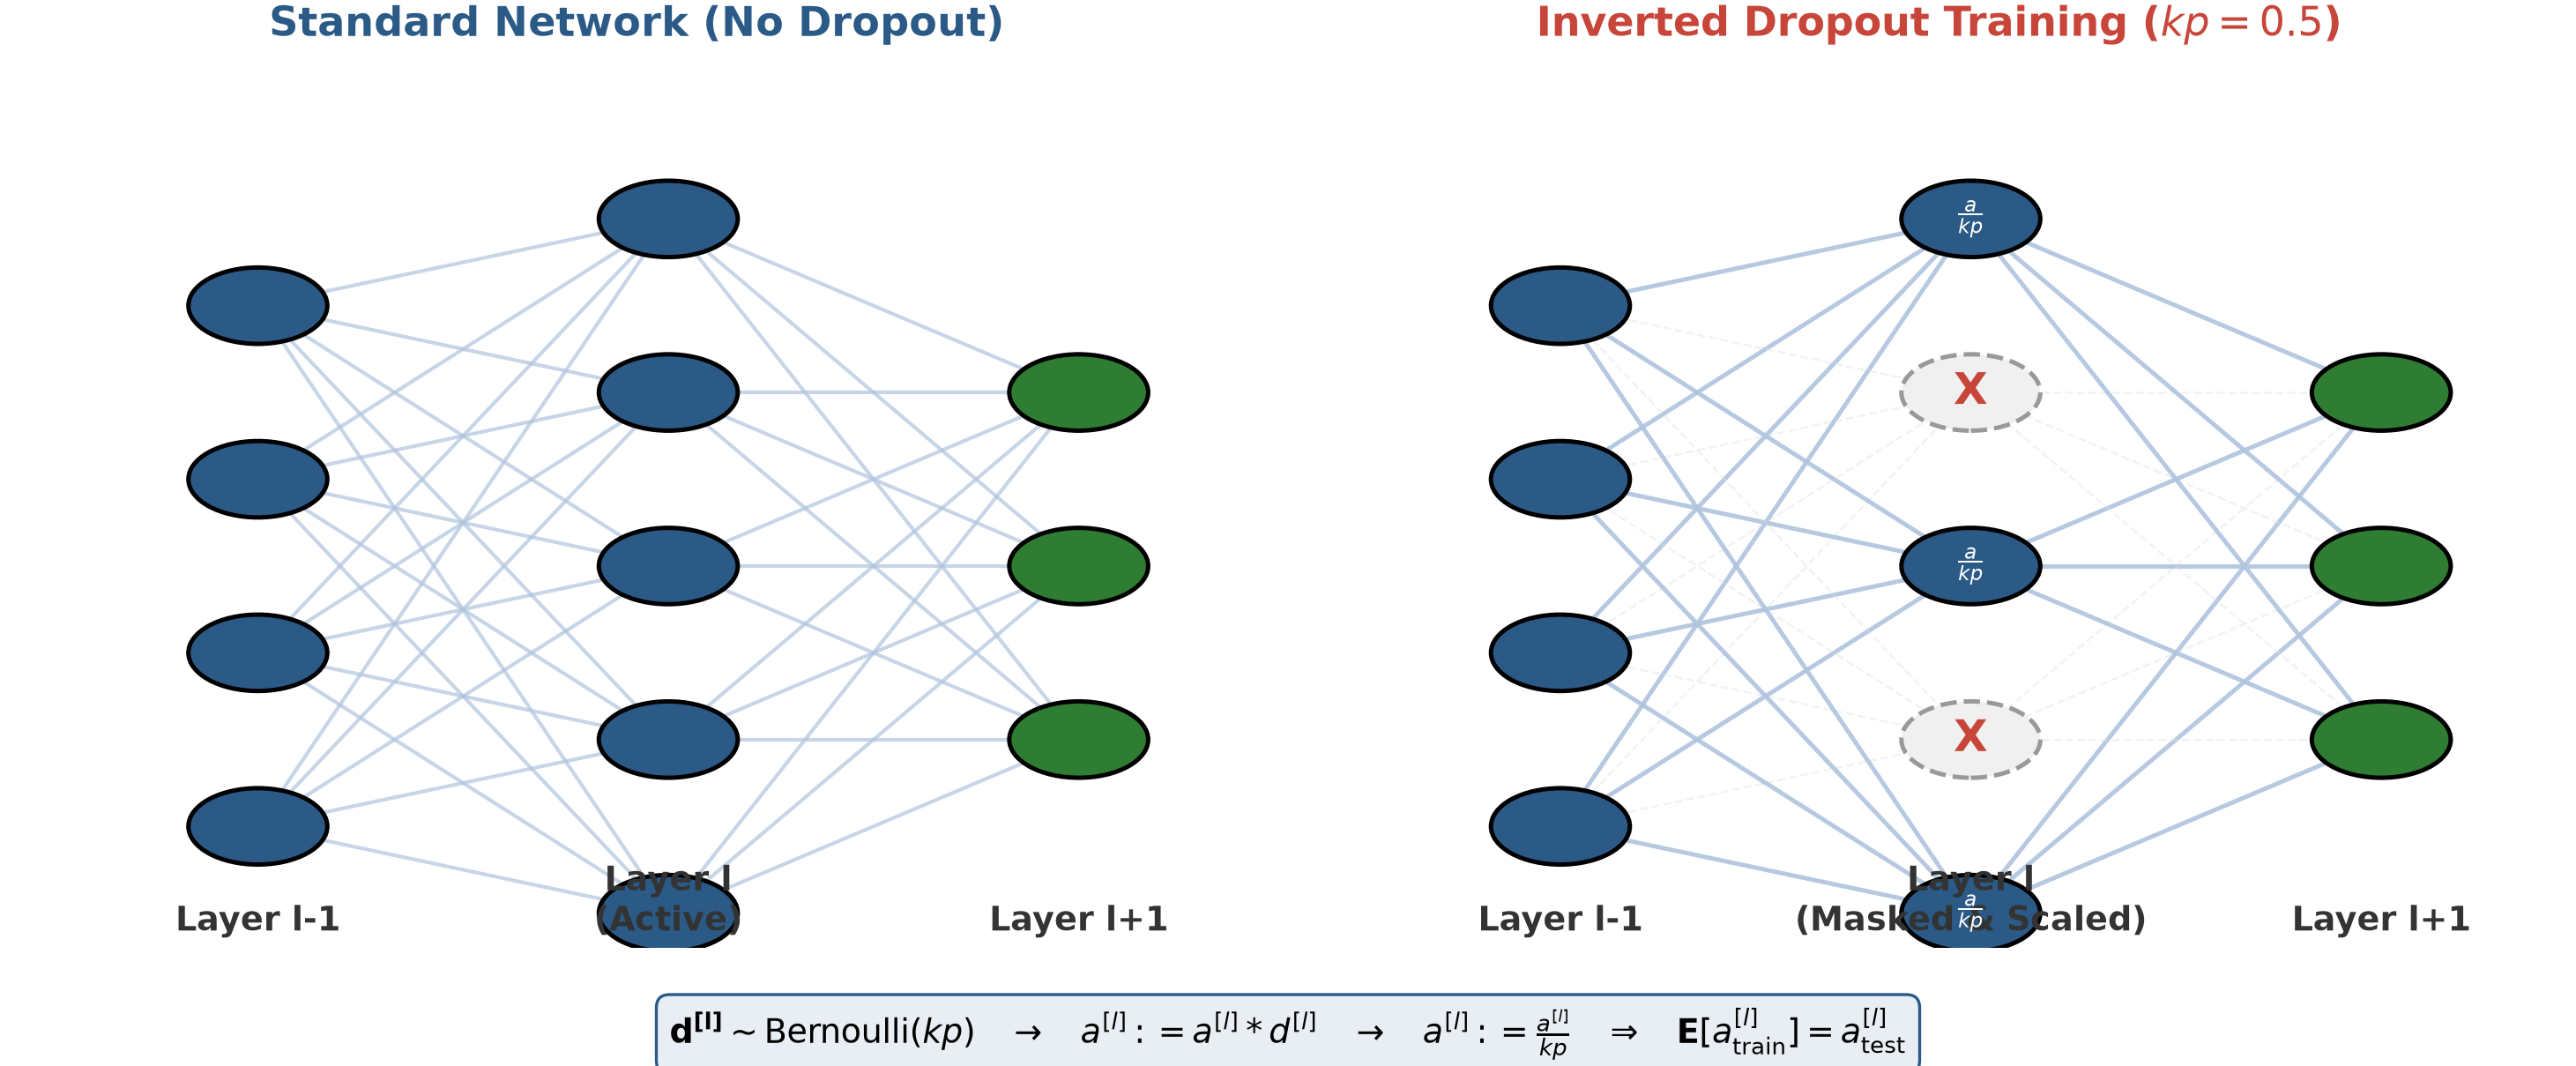
\includegraphics[width=0.68\textwidth]{nn2_dropout.png}\\[-1pt]
{\footnotesize\textit{Inverted Dropout: Generating mask vector $d^{[l]}$, zeroing out dropped units, and scaling by $1/kp$.}}
\end{center}

\vspace{-6pt}

% Step-by-Step Mathematical Mechanics Box
\begin{tcolorbox}[
    colframe=themeblue, colback=lightbg, coltitle=white,
    fonttitle=\bfseries\sffamily\small,
    title={Implementation: Inverted Dropout (3 Simple Steps)},
    arc=1.3mm, boxrule=0.5pt, left=5pt, right=5pt, top=2pt, bottom=2pt
]
\footnotesize
For each layer $l$ during training, Inverted Dropout is implemented in 3 steps:
\begin{enumerate}[leftmargin=12pt, itemsep=1.5pt, topsep=1pt]
    \item \textbf{Generate Random Mask:} Draw a boolean mask $d^{[l]}$ where each entry is $1$ with probability $kp$:
    \[
    d^{[l]} = (\text{np.random.rand}(*a^{[l]}\text{.shape}) < kp)
    \]
    \item \textbf{Zero Out Neurons:} Multiply activations element-wise:
    \[
    a^{[l]} := a^{[l]} * d^{[l]}
    \]
    \item \textbf{Scale Up (Inverted Step):} Divide by the keep probability $kp$:
    \[
    a^{[l]} := \frac{a^{[l]}}{kp}
    \]
\end{enumerate}
\hrulefill\\[1pt]
\textbf{Why Divide by $kp$? (Expected Value Preservation):}
Since dropout zeroes out a fraction $(1 - kp)$ of the neurons, the total signal sum entering the next layer would drop by $(1 - kp)$ without scaling. Dividing by $kp$ restores the original expected value:
\[
\mathbb{E}[a^{[l]}_{\text{dropout}}] = kp \cdot a^{[l]} + (1 - kp) \cdot 0 = kp \cdot a^{[l]} \quad\Longrightarrow\quad \mathbb{E}\left[\frac{a^{[l]} * d^{[l]}}{kp}\right] = a^{[l]}
\]
\textbf{What to do at Test Time? Absolutely Nothing!}
Because activations were already scaled up during training, at test time we use the \textbf{full unmasked network} with standard activations: $a^{[l]} = g(z^{[l]})$. No dropout, no scaling!
\end{tcolorbox}

\vspace{-2pt}

% Intuition Box
\begin{tcolorbox}[
    colframe=accentred, colback=white, arc=1.3mm, boxrule=0.5pt,
    left=5pt, right=5pt, top=2pt, bottom=2pt
]
\footnotesize
\textbf{Why Does Dropout Work? (Two Intuitive Explanations):}
\begin{itemize}[leftmargin=8pt, itemsep=1pt, topsep=0pt]
    \item \textbf{1. Ensemble of Smaller Networks:} At each training step, we train a different random sub-network. At test time, using the full network is like averaging the predictions of $2^N$ different models together.
    \item \textbf{2. Spreading the Weights (No Single Feature is Essential):} A neuron cannot rely heavily on any single input feature because that input might be dropped at any time. Therefore, the neuron is forced to spread its weights across all inputs rather than placing high confidence on just one. This has a shrinking effect on weights, very similar to $L_2$ regularization!
\end{itemize}
\end{tcolorbox}

\vspace{-2pt}

\noindent{\bfseries\color{themeblue} Practical Rules for Dropout:}\par
\begin{itemize}[leftmargin=10pt, itemsep=0.5pt, topsep=0pt]
    \item \textbf{Layer-by-Layer Tuning:} We can set a different $kp$ for each layer. For large, wide layers with many parameters, use a lower $kp$ (e.g., $kp = 0.5$). For small layers, use $kp = 0.8$ or $1.0$ (no dropout).
    \item \textbf{Input Layer:} We rarely apply dropout to the input features ($kp = 1.0$ or at most $0.8$).
    \item \textbf{When to Use:} Use dropout \textbf{only when facing Overfitting (High Variance)}. Do not use it if your model is underfitting (High Bias). It is especially popular in Computer Vision.
\end{itemize}

\newpage

% =========================================================================
% PAGE 2: Data Augmentation & Early Stopping
% =========================================================================

\noindent{\large\bfseries\color{themeblue} 2. Data Augmentation \& Early Stopping}\par\vspace{1pt}
Two other very common and practical ways to regularize a neural network are: adding synthetic data, and stopping training before the model overfits.

\vspace{1pt}

\noindent{\bfseries\color{themeblue} 2.1 Data Augmentation}\par
\begin{itemize}[leftmargin=10pt, itemsep=1pt, topsep=0.5pt]
    \item \textbf{Motivation:} The best cure for overfitting is having more training data. When collecting new data is too hard or expensive, we artificially generate new examples from existing data.
    \item \textbf{Common Image Transformations:}
    \begin{itemize}[leftmargin=8pt, itemsep=0.5pt]
        \item \textit{Horizontal / Vertical Flip:} A flipped image of a cat is still clearly a cat.
        \item \textit{Random Rotations:} Rotate images slightly ($\pm 10^\circ - 30^\circ$) so the model recognizes tilted objects.
        \item \textit{Random Brightness \& Contrast:} Simulates different lighting and camera sensors.
        \item \textit{Random Zoom \& Crop:} Teaches the model to recognize objects whether zoomed in or far away.
    \end{itemize}
    \item \textbf{Why it regularizes:} It prevents the network from memorizing specific pixel coordinates and forces it to learn real, invariant visual features.
    \item \textbf{Implementation:} Done on-the-fly during training batches using \texttt{ImageDataGenerator} in Keras or modern layers (\texttt{RandomFlip}, \texttt{RandomRotation}).
\end{itemize}

\vspace{-2pt}

\begin{center}
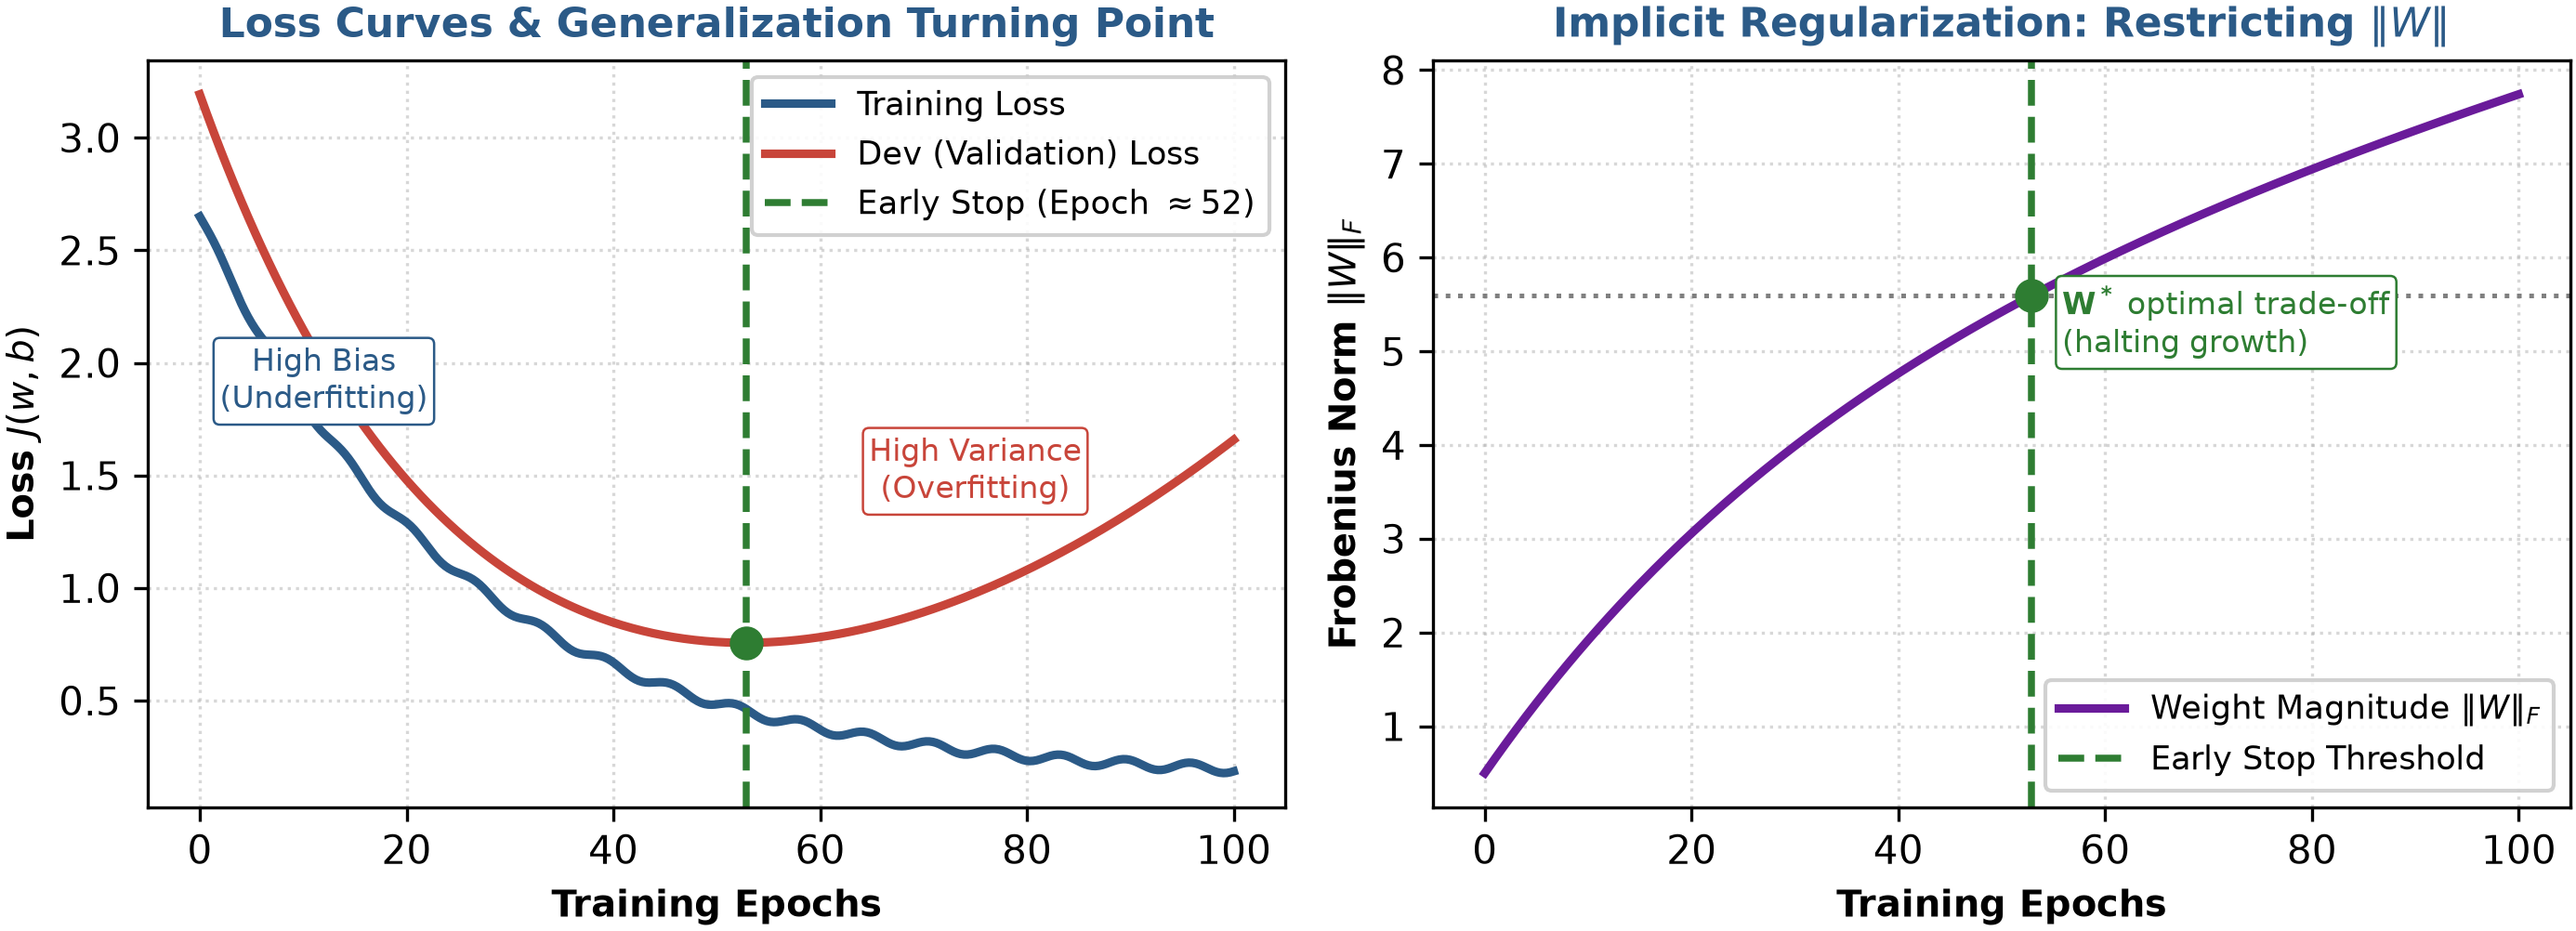
\includegraphics[width=0.82\textwidth]{nn2_early_stopping.png}\\[-1pt]
{\footnotesize\textit{Early Stopping: Stopping at the minimum of the validation loss curve prevents weights from growing too large.}}
\end{center}

\vspace{-6pt}

\noindent{\bfseries\color{themeblue} 2.2 Early Stopping}\par
During training, the training loss continuously goes down. But the validation (dev) loss goes down at first, reaches a minimum, and then starts going back up as the model begins overfitting:
\begin{enumerate}[leftmargin=12pt, itemsep=0.5pt, topsep=0.5pt]
    \item \textbf{Underfitting Phase:} Training and dev loss both decrease rapidly.
    \item \textbf{Best Stopping Point:} Dev loss reaches its lowest point (best generalization).
    \item \textbf{Overfitting Phase:} Training loss keeps falling, but dev loss increases because the network is memorizing noise.
\end{enumerate}

\vspace{-2pt}

% Connection to L2 Box
\begin{tcolorbox}[
    colframe=themeblue, colback=lightbg, arc=1.3mm, boxrule=0.5pt,
    left=5pt, right=5pt, top=2pt, bottom=2pt
]
\footnotesize
\textbf{Why Does Early Stopping Act Like $L_2$ Regularization?}
\begin{itemize}[leftmargin=8pt, itemsep=0.5pt, topsep=0pt]
    \item Weights $W$ start initialized near zero ($\|W\| \approx 0$).
    \item With each gradient descent step, weights grow in size to fit more complex patterns.
    \item By stopping training early, we \textbf{prevent weights from becoming large}.
    \item In fact, stopping after $T$ iterations is mathematically very similar to applying $L_2$ regularization with penalty parameter $\lambda \approx 1 / (\alpha T)$. Both restrict the size of weights!
\end{itemize}
\end{tcolorbox}

\vspace{-2pt}

% Orthogonalization Box
\begin{tcolorbox}[
    colframe=accentred, colback=white, coltitle=white,
    fonttitle=\bfseries\sffamily\small,
    title={The Orthogonalization Trade-off: Early Stopping vs. $L_2$ Regularization},
    arc=1.3mm, boxrule=0.5pt, left=5pt, right=5pt, top=2pt, bottom=2pt
]
\footnotesize
\textbf{The Orthogonalization Principle:} In machine learning, it is ideal to have separate controls for separate tasks:
\begin{itemize}[leftmargin=8pt, itemsep=0.5pt, topsep=0pt]
    \item \textit{Task 1 (Minimize Cost $J$ on Train Set):} Use optimizers (Adam, RMSProp), train longer, or use a larger model.
    \item \textit{Task 2 (Prevent Overfitting on Dev Set):} Use regularization ($L_2$, Dropout) or add more data.
\end{itemize}
\hrulefill\\[1pt]
\textbf{Comparison:}
\begin{itemize}[leftmargin=8pt, itemsep=0.5pt, topsep=0pt]
    \item \textbf{Early Stopping Violates Orthogonalization:} Stopping early stops you from minimizing training loss (hurts Task 1) in order to prevent dev error from rising (helps Task 2). You affect both tasks with one single knob!
    \item \textbf{Advantage of Early Stopping:} You only need to run training \textbf{once}. With $L_2$, you have to train multiple times to test different values of $\lambda$.
\end{itemize}
\end{tcolorbox}

\newpage

% =========================================================================
% PAGE 3: Vanishing & Exploding Gradients & Symmetry Breaking
% =========================================================================

\noindent{\large\bfseries\color{themeblue} 3. Vanishing and Exploding Gradients in Deep Networks}\par\vspace{1pt}
When a neural network has many layers ($L$ is large), activations and gradients can grow or shrink exponentially with depth.

\vspace{-2pt}

% Mathematical Proof Box
\begin{tcolorbox}[
    colframe=themeblue, colback=lightbg, coltitle=white,
    fonttitle=\bfseries\sffamily\small,
    title={Simple Mathematical Example: Exponential Compounding with Depth},
    arc=1.3mm, boxrule=0.5pt, left=5pt, right=5pt, top=2pt, bottom=2pt
]
\footnotesize
Imagine a deep network with $L$ layers, no bias ($b = 0$), linear activations ($g(z) = z$), and weight matrices scaled by a constant factor $p$:
\[
W^{[l]} = \begin{bmatrix} p & 0 \\ 0 & p \end{bmatrix} = p \cdot I
\]
The output after $L$ layers is:
\[
\hat{y} = W^{[L]} W^{[L-1]} \cdots W^{[1]} x = (p \cdot I)^L x = p^L x
\]
\textbf{What happens as depth $L$ grows? (e.g., $L = 50$ layers):}
\begin{itemize}[leftmargin=8pt, itemsep=0.5pt, topsep=0pt]
    \item \textbf{If $p > 1$ (e.g., $p = 1.5$):}
    $p^L = (1.5)^{50} \approx 6.37 \times 10^8$. Signals and gradients blow up exponentially $\implies$ \textbf{Exploding Gradients}. Leads to numerical overflow (\texttt{NaN}) and unstable training.
    \item \textbf{If $p < 1$ (e.g., $p = 0.5$):}
    $p^L = (0.5)^{50} \approx 8.88 \times 10^{-16}$. Signals and gradients vanish exponentially $\implies$ \textbf{Vanishing Gradients}. Gradients in the early layers become virtually zero, and early layers stop learning completely!
\end{itemize}
\end{tcolorbox}

\vspace{-3pt}

\begin{center}
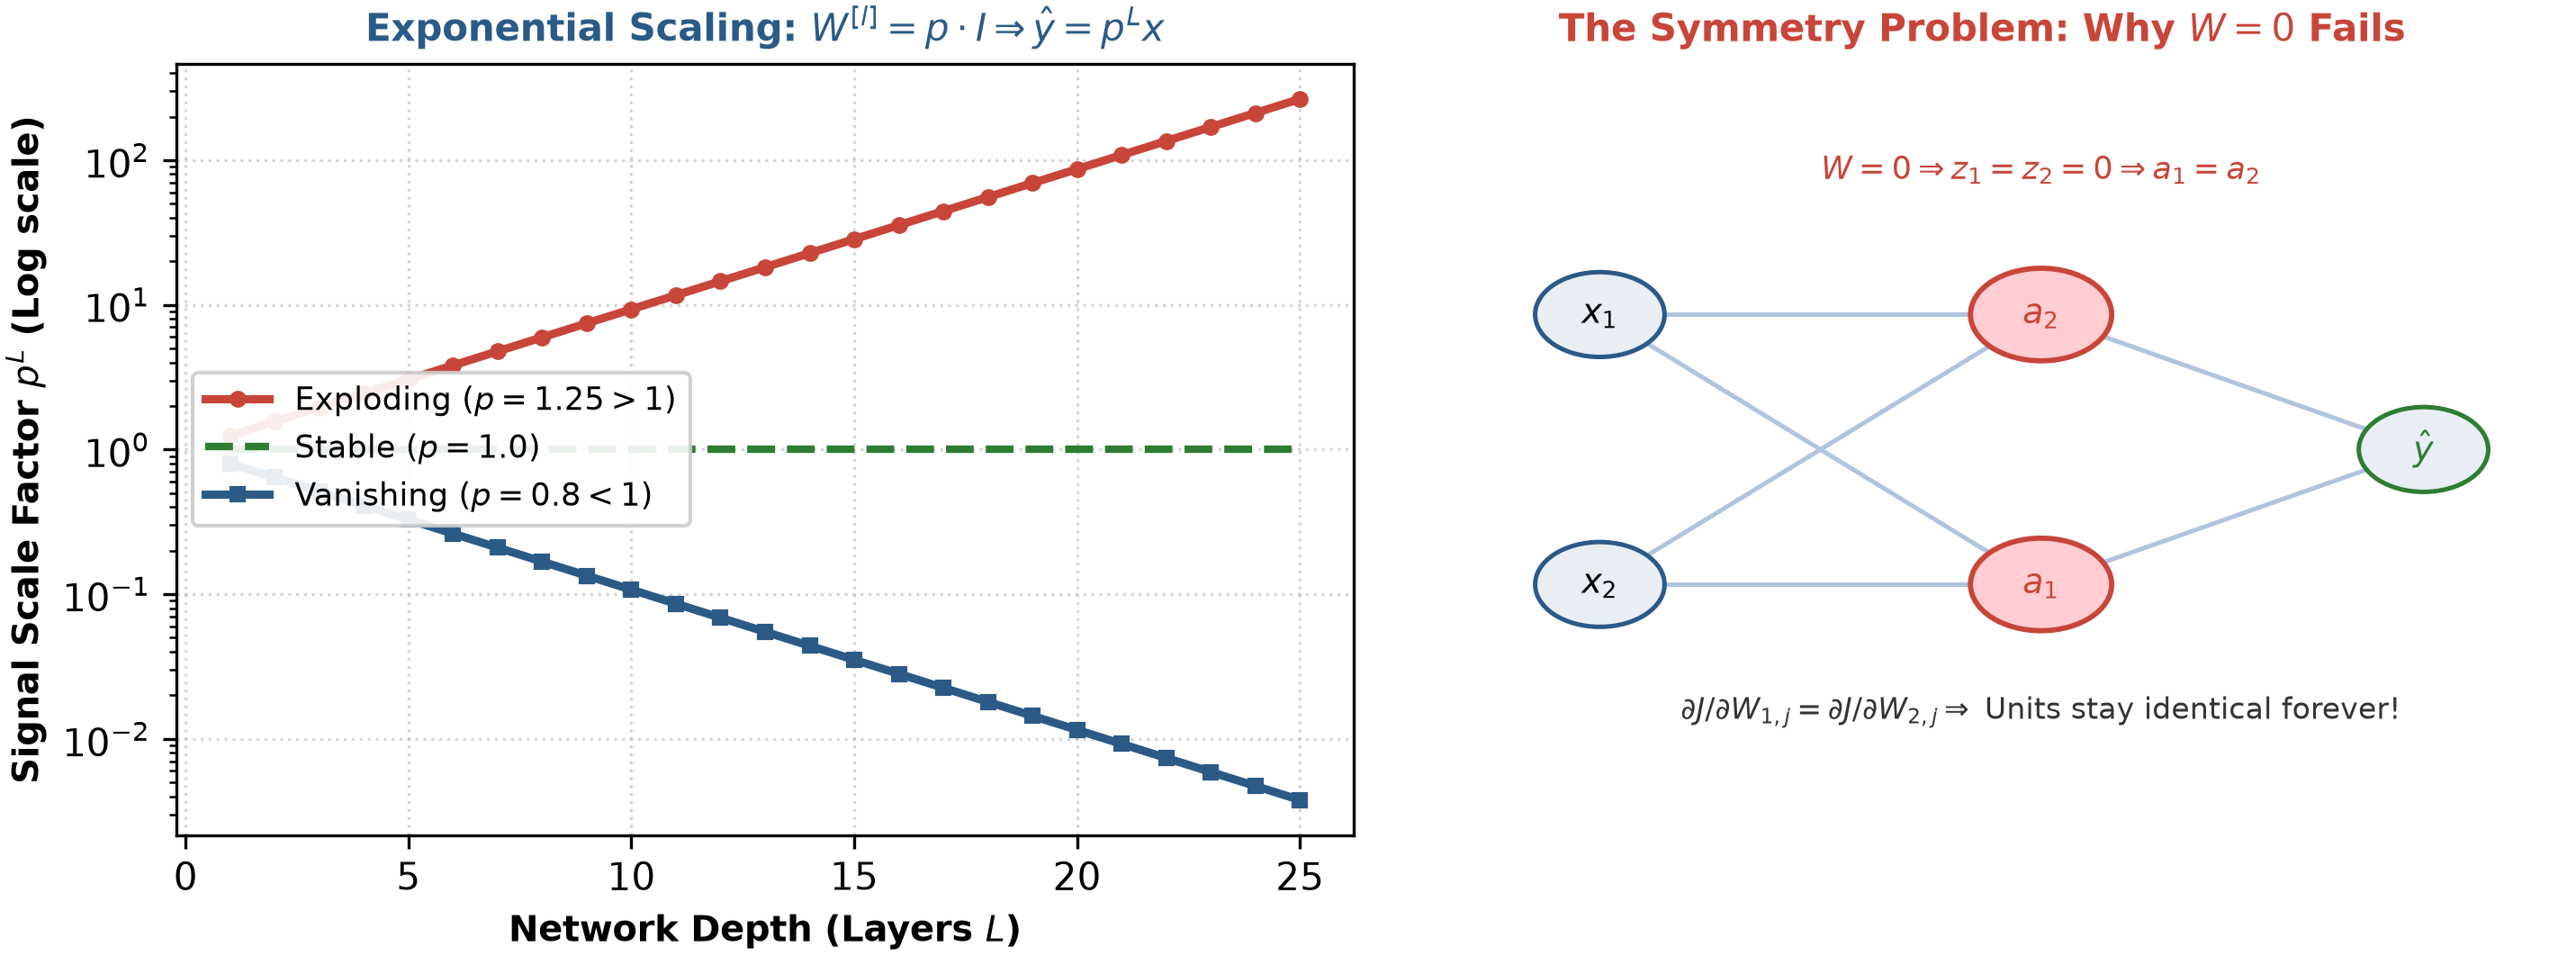
\includegraphics[width=0.82\textwidth]{nn2_vanishing_exploding.png}\\[-1pt]
{\footnotesize\textit{Left: Compounding factor $p^L$ across layers. Right: Why zero initialization ($W = 0$) causes the Symmetry Problem.}}
\end{center}

\vspace{-6pt}

\noindent{\bfseries\color{themeblue} The Symmetry Problem: Why We Cannot Initialize Weights to Zero}\par
In Logistic Regression, initializing weights to zero ($w = 0, b = 0$) works fine. But in a Neural Network, \textbf{initializing hidden layer weights to zero causes complete failure}:

\begin{tcolorbox}[
    colframe=accentred, colback=white, arc=1.3mm, boxrule=0.5pt,
    left=5pt, right=5pt, top=2pt, bottom=2pt
]
\footnotesize
\textbf{Why Does Zero Initialization Fail? (Step-by-Step Proof):}
Suppose we initialize a layer's weights and biases to zero: $W = 0, b = 0$:
\begin{enumerate}[leftmargin=12pt, itemsep=1pt, topsep=0pt]
    \item \textbf{Identical Activations:} All hidden neurons compute $z_1 = z_2 = 0 \implies a_1 = a_2 = g(0)$.
    \item \textbf{Identical Gradients:} Downstream layers receive identical signals, so backpropagation calculates the exact same gradient for all incoming weights: $\frac{\partial J}{\partial W_{1, j}} = \frac{\partial J}{\partial W_{2, j}}$.
    \item \textbf{Identical Updates:} After gradient descent, $W_{1, j}$ and $W_{2, j}$ remain exactly equal: $W_{1, j} = W_{2, j}$.
\end{enumerate}
\textbf{Consequence:} All hidden neurons compute the exact same feature! No matter how many neurons you add, the layer acts as if it has only \textbf{one single neuron}.
\\[1pt]
\textbf{Why Did Zero Work for Logistic Regression?} Logistic regression has only 1 output unit. There are no other hidden units to be symmetric with!
\\[1pt]
\textbf{Solution:} Weights in neural networks \textbf{must be initialized randomly} to break symmetry.
\end{tcolorbox}

\vspace{-2pt}

\noindent{\bfseries\color{themeblue} Small Random Initialization (\texttt{np.random.randn(...) * 0.01}):}\par
\begin{itemize}[leftmargin=10pt, itemsep=0.5pt, topsep=0.5pt]
    \item \textbf{Why small?} For Sigmoid and Tanh, small weights keep $z$ near zero where the slope is steepest ($g'(0) = 1$ for tanh), avoiding flat saturation zones.
    \item \textbf{Why 0.01 fails in deep networks:} A fixed number like $0.01$ causes signals to vanish when multiplied across 20 or 50 layers. We need weight scales that adjust automatically to the size of the layer!
\end{itemize}

\newpage

% =========================================================================
% PAGE 4: Deducing Xavier & He Initializers
% =========================================================================

\noindent{\large\bfseries\color{themeblue} 4. Weight Initialization Theory: Deducing Xavier \& He}\par\vspace{1pt}
To prevent vanishing and exploding gradients, our goal is simple: \textbf{preserve the signal variance from layer to layer}, so that the variance of the output $z$ equals the variance of the input $x$ ($\mathbf{\text{Var}(z) = \text{Var}(x)}$).

\vspace{-2pt}

% General Variance Formula Box
\begin{tcolorbox}[
    colframe=themeblue, colback=lightbg, coltitle=white,
    fonttitle=\bfseries\sffamily\small,
    title={The Fundamental Rule: Preserving Signal Variance ($\text{Var}(z) = \text{Var}(x)$)},
    arc=1.3mm, boxrule=0.5pt, left=5pt, right=5pt, top=2pt, bottom=2pt
]
\footnotesize
Consider a single neuron computing $z = w_1 x_1 + w_2 x_2 + \dots + w_n x_n$ (with $n = n^{[l-1]}$ inputs and $b = 0$).
\\[1pt]
Assuming weights $w_i$ and inputs $x_i$ are independent with mean zero:
\[
\text{Var}(w_i x_i) = \text{Var}(w_i) \cdot \text{Var}(x_i) = \text{Var}(w) \cdot \text{Var}(x)
\]
Since $z$ is the sum of $n$ independent inputs:
\[
\text{Var}(z) = \sum_{i=1}^n \text{Var}(w_i x_i) = n \cdot \text{Var}(w) \cdot \text{Var}(x)
\]
\textbf{The Golden Rule:} We want the signal variance neither to explode nor to vanish across layers. Therefore, we enforce:
\[
\mathbf{\text{Var}(z) \stackrel{!}{=} \text{Var}(x)} \quad\Longrightarrow\quad n \cdot \text{Var}(w) \cdot \text{Var}(x) = \text{Var}(x) \quad\Longrightarrow\quad \mathbf{n \cdot \text{Var}(w) = 1}
\]
From this single rule, we directly deduce both Xavier and He initializations!
\end{tcolorbox}

\vspace{-3pt}

\begin{center}
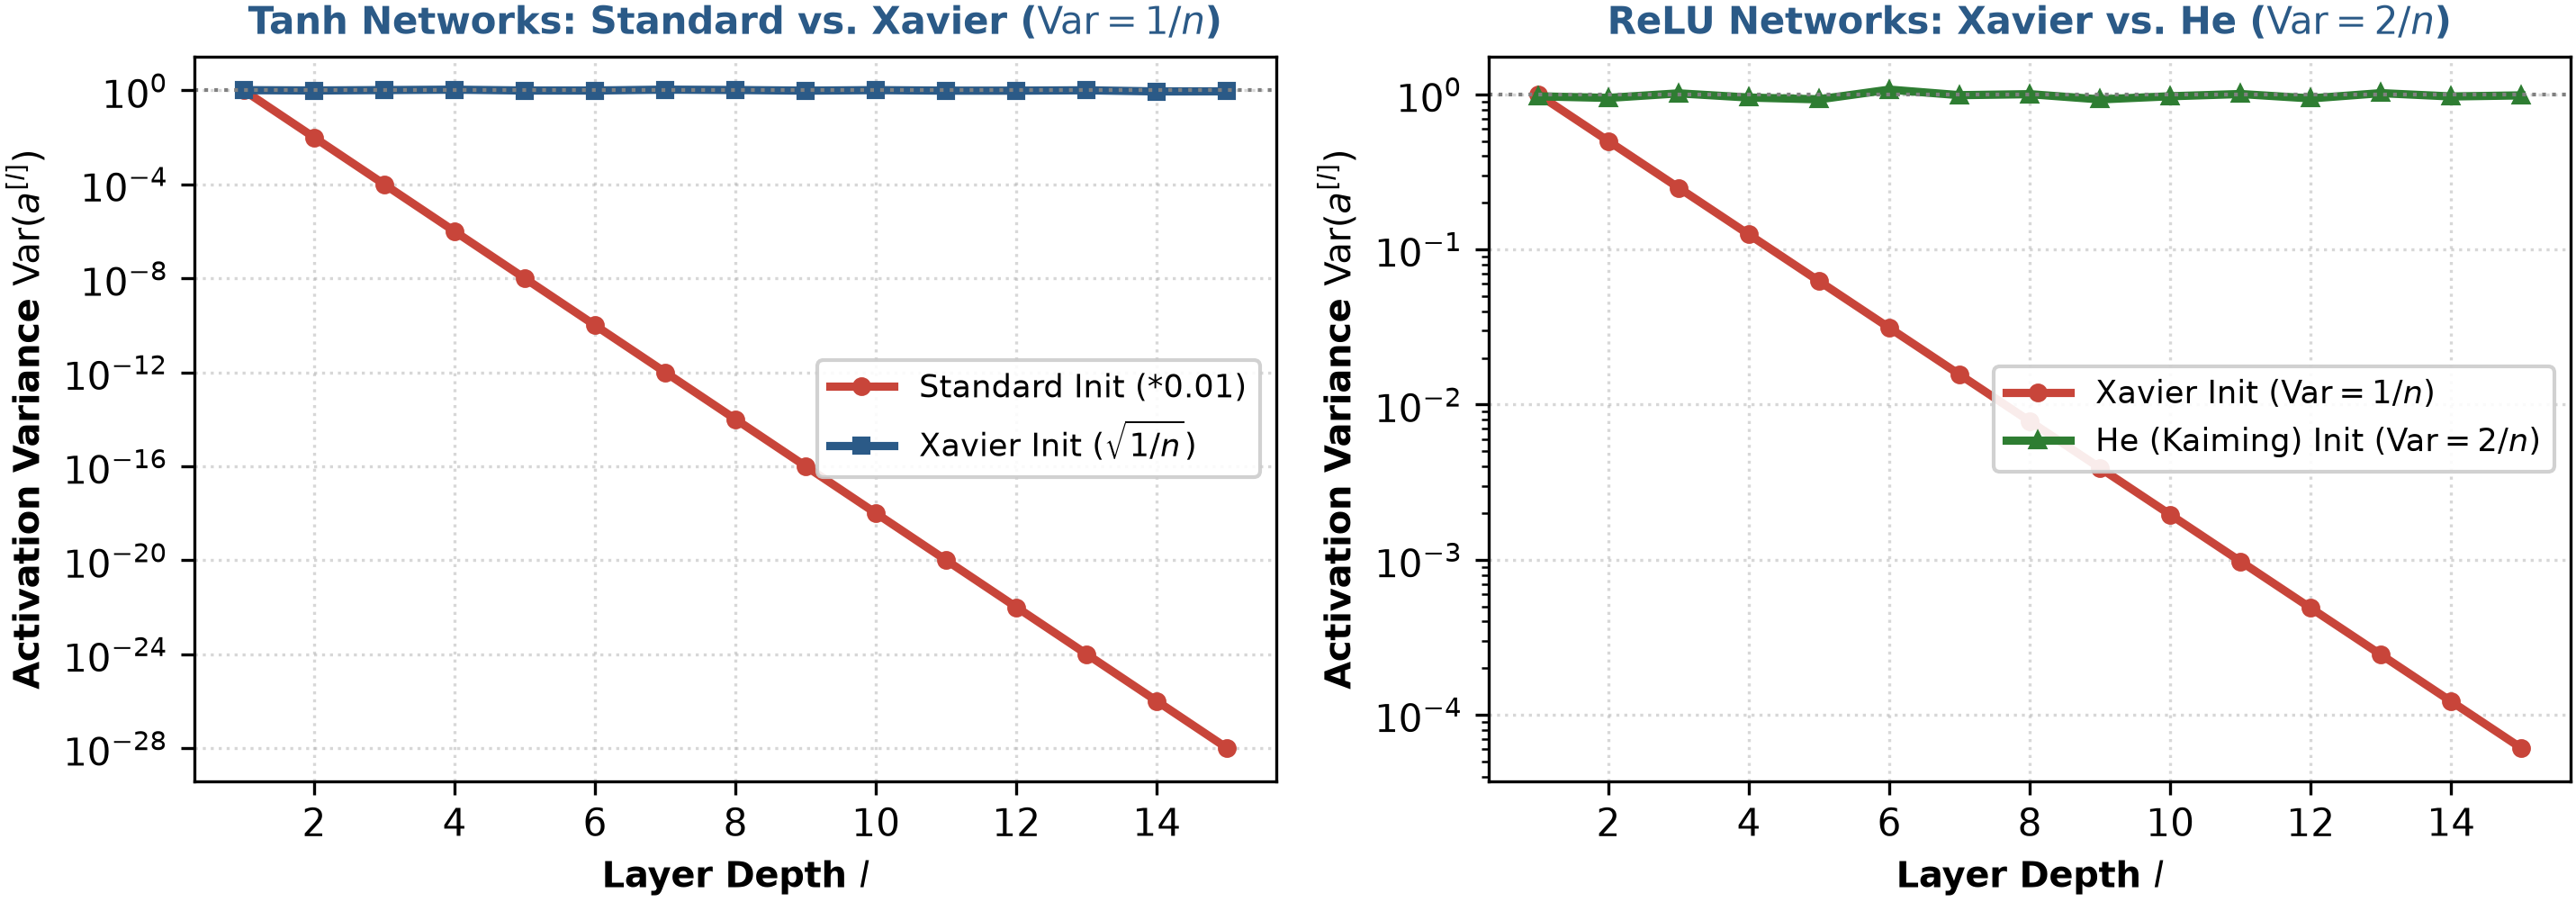
\includegraphics[width=0.82\textwidth]{nn2_initialization_variance.png}\\[-1pt]
{\footnotesize\textit{Variance preservation: Xavier maintains $\text{Var}=1$ for Tanh; He maintains $\text{Var}=1$ for ReLU by doubling weight variance to $2/n$.}}
\end{center}

\vspace{-6pt}

% Deduction of Xavier and He side-by-side
\noindent\begin{minipage}[t]{0.485\textwidth}
\begin{tcolorbox}[
    colframe=themeblue, colback=lightbg, coltitle=white,
    fonttitle=\bfseries\sffamily\small,
    title={1. Deducing Xavier Initialization (Tanh)},
    arc=1.3mm, boxrule=0.5pt, left=4pt, right=4pt, top=2pt, bottom=2pt
]
\footnotesize
\textbf{Target Activations:} Tanh \& Sigmoid.
\\[1.5pt]
\textbf{Deduction:}
For Tanh near zero, $\tanh(z) \approx z$, so the activation does not reduce the variance ($\text{Var}(a) \approx \text{Var}(z)$).
\\[1.5pt]
Applying our rule $n \cdot \text{Var}(w) = 1$:
\[
\mathbf{\text{Var}(w) = \frac{1}{n}} \quad\Longrightarrow\quad \mathbf{\sigma_w = \sqrt{\frac{1}{n^{[l-1]}}}}
\]
\textbf{NumPy Code:}
\begin{verbatim}
W = np.random.randn(n_l, n_in) \
    * np.sqrt(1.0 / n_in)
\end{verbatim}
\textbf{Normalized Xavier (Glorot \& Bengio 2010):}
Averaging fan-in ($n_{\text{in}}$) and fan-out ($n_{\text{out}}$):
\[
\text{Var}(w) = \frac{2}{n_{\text{in}} + n_{\text{out}}}
\]
\end{tcolorbox}
\end{minipage}
\hfill
\begin{minipage}[t]{0.485\textwidth}
\begin{tcolorbox}[
    colframe=accentgreen, colback=white, coltitle=white,
    fonttitle=\bfseries\sffamily\small,
    title={2. Deducing He Initialization (ReLU)},
    arc=1.3mm, boxrule=0.5pt, left=4pt, right=4pt, top=2pt, bottom=2pt
]
\footnotesize
\textbf{Target Activations:} ReLU \& Leaky ReLU.
\\[1.5pt]
\textbf{Deduction (Why the Factor of 2?):}
ReLU sets all negative inputs to zero ($a = \max(0, z)$). This zeroes out half the distribution, \textbf{cutting the variance in half}:
\[
\text{Var}(a) = \frac{1}{2}\text{Var}(z)
\]
When $a$ becomes the input to the next layer:
\[
\text{Var}(z_{\text{next}}) = n \cdot \text{Var}(w) \cdot \left(\frac{1}{2}\text{Var}(z)\right) = \frac{n}{2} \cdot \text{Var}(w) \cdot \text{Var}(z)
\]
To preserve variance ($\text{Var}(z_{\text{next}}) \stackrel{!}{=} \text{Var}(z)$):
\[
\frac{n}{2} \cdot \text{Var}(w) = 1 \quad\Longrightarrow\quad \mathbf{\text{Var}(w) = \frac{2}{n}} \quad\Longrightarrow\quad \mathbf{\sigma_w = \sqrt{\frac{2}{n^{[l-1]}}}}
\]
\textbf{NumPy Code (He et al. 2015):}
\begin{verbatim}
W = np.random.randn(n_l, n_in) \
    * np.sqrt(2.0 / n_in)
\end{verbatim}
\end{tcolorbox}
\end{minipage}

\vspace{1pt}

% Master Reference Table
\noindent{\bfseries\color{themeblue} Master Summary: Weight Initialization Reference Table}\par\vspace{1pt}
\begin{center}
\footnotesize
\setlength{\tabcolsep}{4pt}
\begin{tabularx}{\textwidth}{p{0.21\textwidth}p{0.18\textwidth}p{0.17\textwidth}>{\raggedright\arraybackslash}X}
\toprule
\rowcolor{lightbg}
\textbf{Activation Function} & \textbf{Initialization Name} & \textbf{Variance Formula} & \textbf{NumPy Implementation Code} \\
\midrule
\textbf{Tanh / Sigmoid} & Xavier (Glorot) & $\text{Var}(W) = \frac{1}{n^{[l-1]}}$ & \texttt{W = np.random.randn(n\_l, n\_in) * np.sqrt(1/n\_in)} \\
\midrule
\textbf{Tanh / Sigmoid (Alt)} & Normalized Xavier & $\text{Var}(W) = \frac{2}{n_{\text{in}} + n_{\text{out}}}$ & \texttt{W = np.random.randn(n\_l, n\_in) * np.sqrt(2/(n\_in + n\_l))} \\
\midrule
\textbf{ReLU / Leaky ReLU} & He (Kaiming) & $\text{Var}(W) = \frac{2}{n^{[l-1]}}$ & \texttt{W = np.random.randn(n\_l, n\_in) * np.sqrt(2/n\_in)} \\
\midrule
\textbf{Biases ($b^{[l]}$)} & Zeros & $\text{Var}(b) = 0$ & \texttt{b = np.zeros((n\_l, 1))} \textit{(Symmetry broken by $W$)} \\
\bottomrule
\end{tabularx}
\end{center}

\end{document}
